\documentclass{article}
\usepackage{graphicx}
\usepackage{epstopdf}
\usepackage{subfigure}
\usepackage{multirow}
\usepackage{wrapfig}
\usepackage{amssymb}
\usepackage{amsfonts, amsmath}
\usepackage{amsmath}
\usepackage{mathrsfs}
\usepackage{enumerate}
% \usepackage[bookmarks=true]{hyperref}
% \usepackage[acronym]{glossaries}
%\usepackage{bookmark}
\usepackage{amssymb,amsmath,amsthm,amsfonts}
\usepackage{mathrsfs}
\usepackage{dsfont}
\usepackage{enumerate}

%\newtheorem{mdef}{Definition}
%\newtheorem{theorem}{Theorem}
\newcommand{\eqsplit}[2]{
  \begin{equation}\label{#2}
    \begin{split}
      #1
    \end{split}
  \end{equation}}
\newcommand{\eqnsplit}[1]{
  \begin{eqnarray*}
    #1
  \end{eqnarray*}}
\newcommand{\tran}[1]{
  \tilde{#1}
}
\newcommand{\td}[2]{
  \frac{d #1}{d #2}
}
\newcommand{\pd}[2]{
  \frac{\partial #1}{\partial #2}
}
\newcommand{\ppd}[2]{
  \frac{\partial^2 #1}{\partial #2^2}
}
\newcommand{\pdd}[3]{
  \frac{\partial^2 #1}{\partial #2 \partial #3}
}
\newcommand{\otd}[1]{
  \frac{d}{d #1}
}
\newcommand{\opd}[1]{
  \frac{\partial}{\partial #1}
}
\newcommand{\oppd}[1]{
  \frac{\partial^2}{\partial #1^2}
}
\newcommand{\opdd}[2]{
  \frac{\partial^2}{\partial #1 \partial #2}
}
\newcommand{\ket}[1]{
  |#1\rangle
}
\newcommand{\bra}[1]{
  \langle#1|
}
\newcommand{\inn}[1]{
  \langle#1\rangle
}
\newcommand{\mean}[1]{
  \langle#1\rangle
}
\newcommand{\tr}{
  \text{tr}\,
}
\newcommand{\re}{
  \text{Re}\,
}
\newcommand\im{
  \text{Im}\,
}
\newcommand{\var}{
  \text{var}
}
\newcommand{\arcsinh}{
  \sinh^{-1}
}
\newcommand{\arccosh}{
  \cosh^{-1}
}
\newcommand{\erfc}{
  \text{erfc}
}
\newcommand{\E}{
  \mathbb{E}
}
\renewcommand{\P}{
  \mathbb{P}
}
\newcommand{\I}[1]{
  \mathbf{1}_{\{#1\}}
}
\newcommand{\1}[1]{
  \mathds{1}_{\{#1\}}
}
\newcommand{\diag}{
  \text{diag\,}
}
\newcommand{\M}{
  {\text{max}}
}
\newcommand{\m}{
  {\text{min}}
}
\newcommand{\ph}{
  {\text{arg}\,}
}
\newcommand\erf{
  \text{erf}
}
\renewcommand\vec[1]{
  \mathbf{#1}
}
\newcommand\mtx[1]{
  \mathbf{#1}
}
\newcommand\ed{
  \,{\buildrel d \over =}\,
}




\DeclareGraphicsExtensions{.eps, .pdf}

\begin{document}
\section{Spectra with same q and different $T$}
The following figure shows the spectra of correlation matrices with
fixed ratio $q = T/N$, and varying $T$ and $N$.
\begin{figure}[htb!]
  \centering
  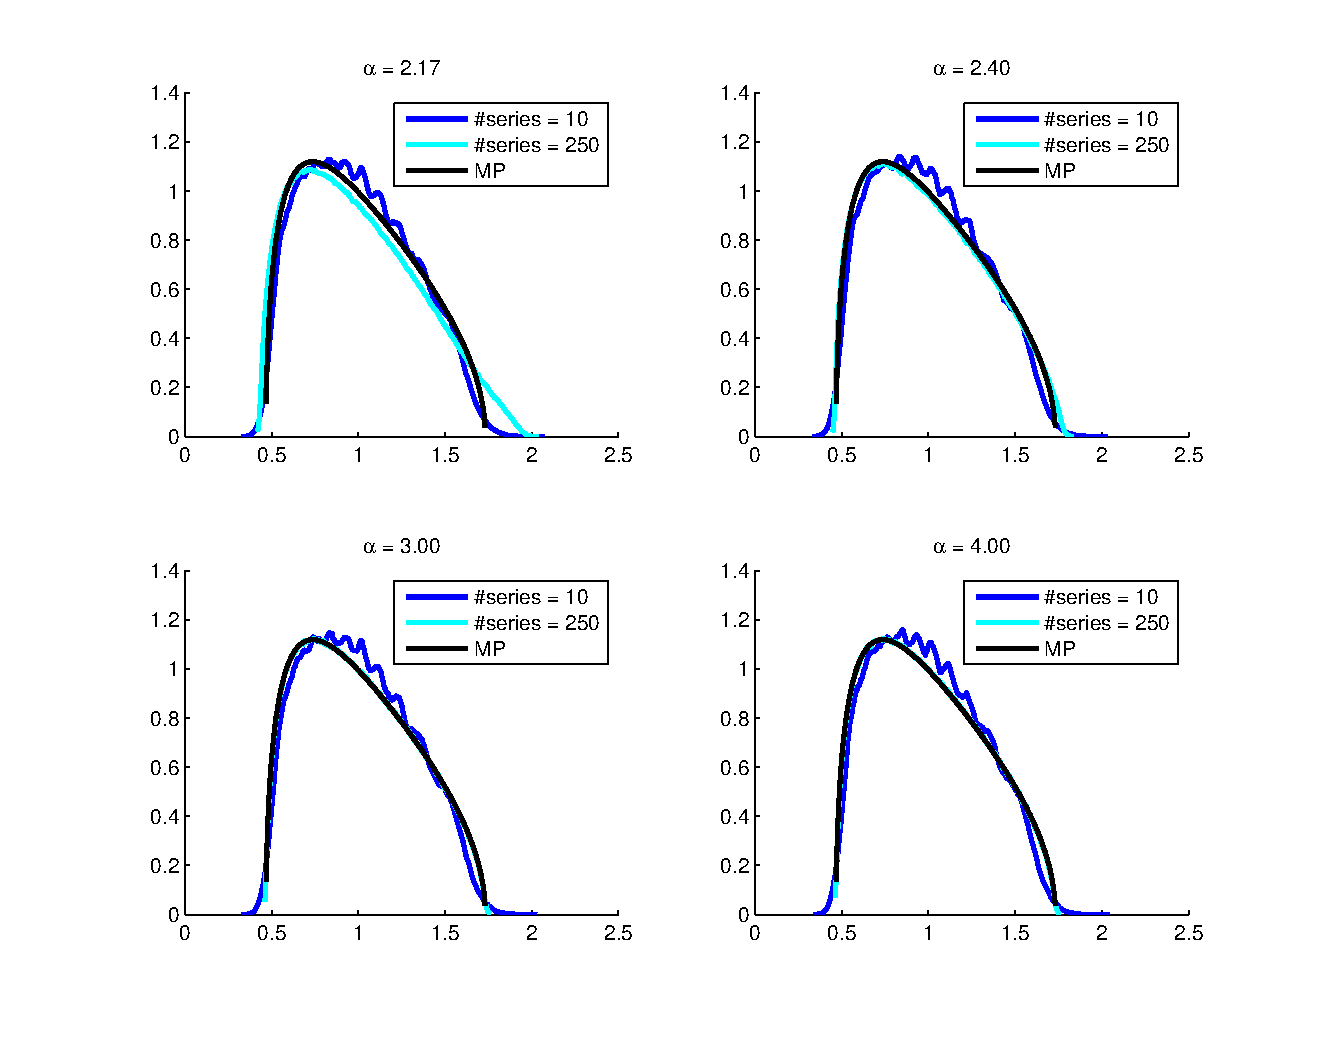
\includegraphics[scale=0.4]{../pics/spectra_q10.eps}
  \caption{\small \it Spectra with q = 10}
\end{figure}

\begin{figure}[htb!]
  \centering
  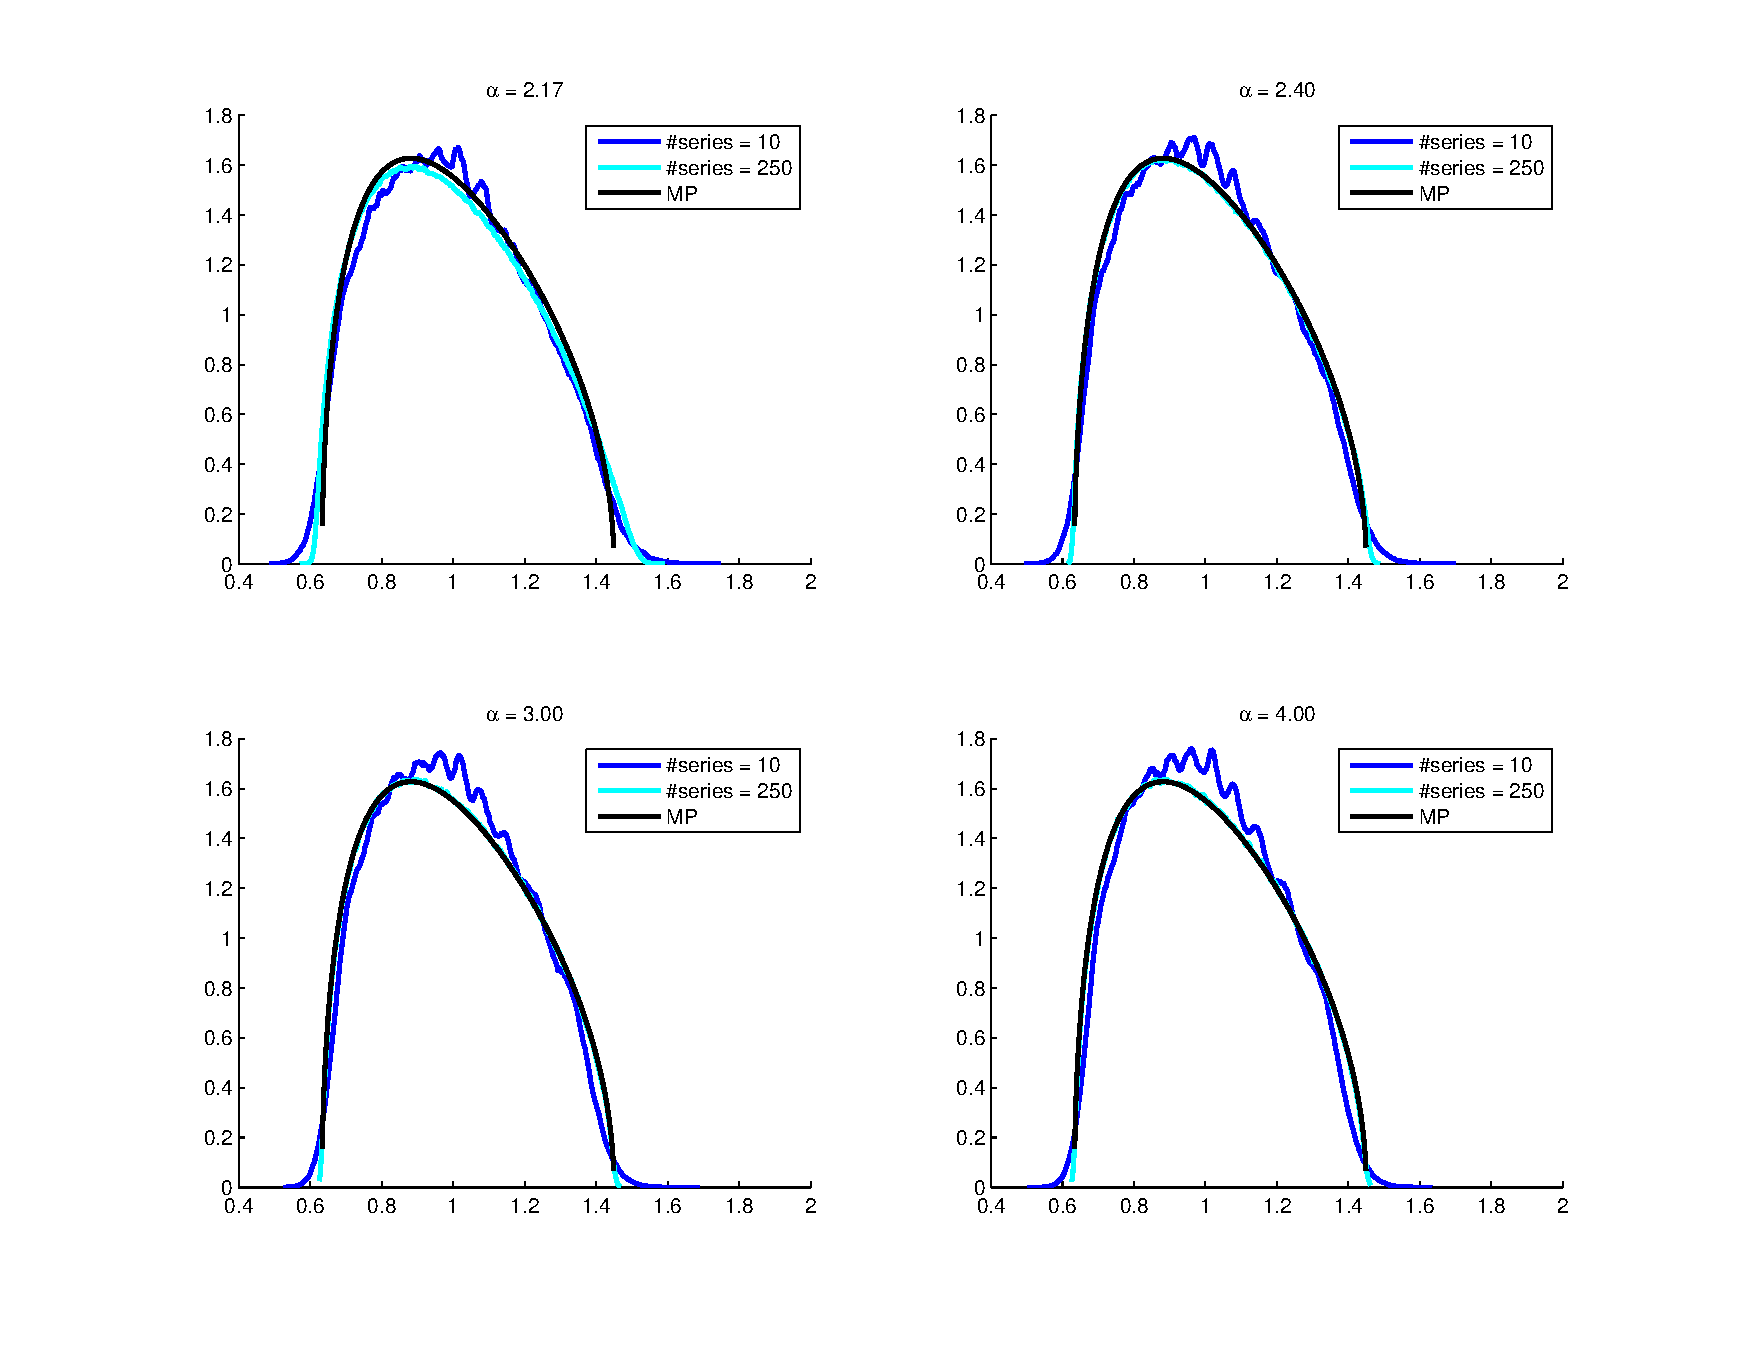
\includegraphics[scale=0.3]{../pics/spectra_q24.eps}
  \caption{\small \it Spectra with q = 24}
\end{figure}

\begin{figure}[htb!]
  \centering
  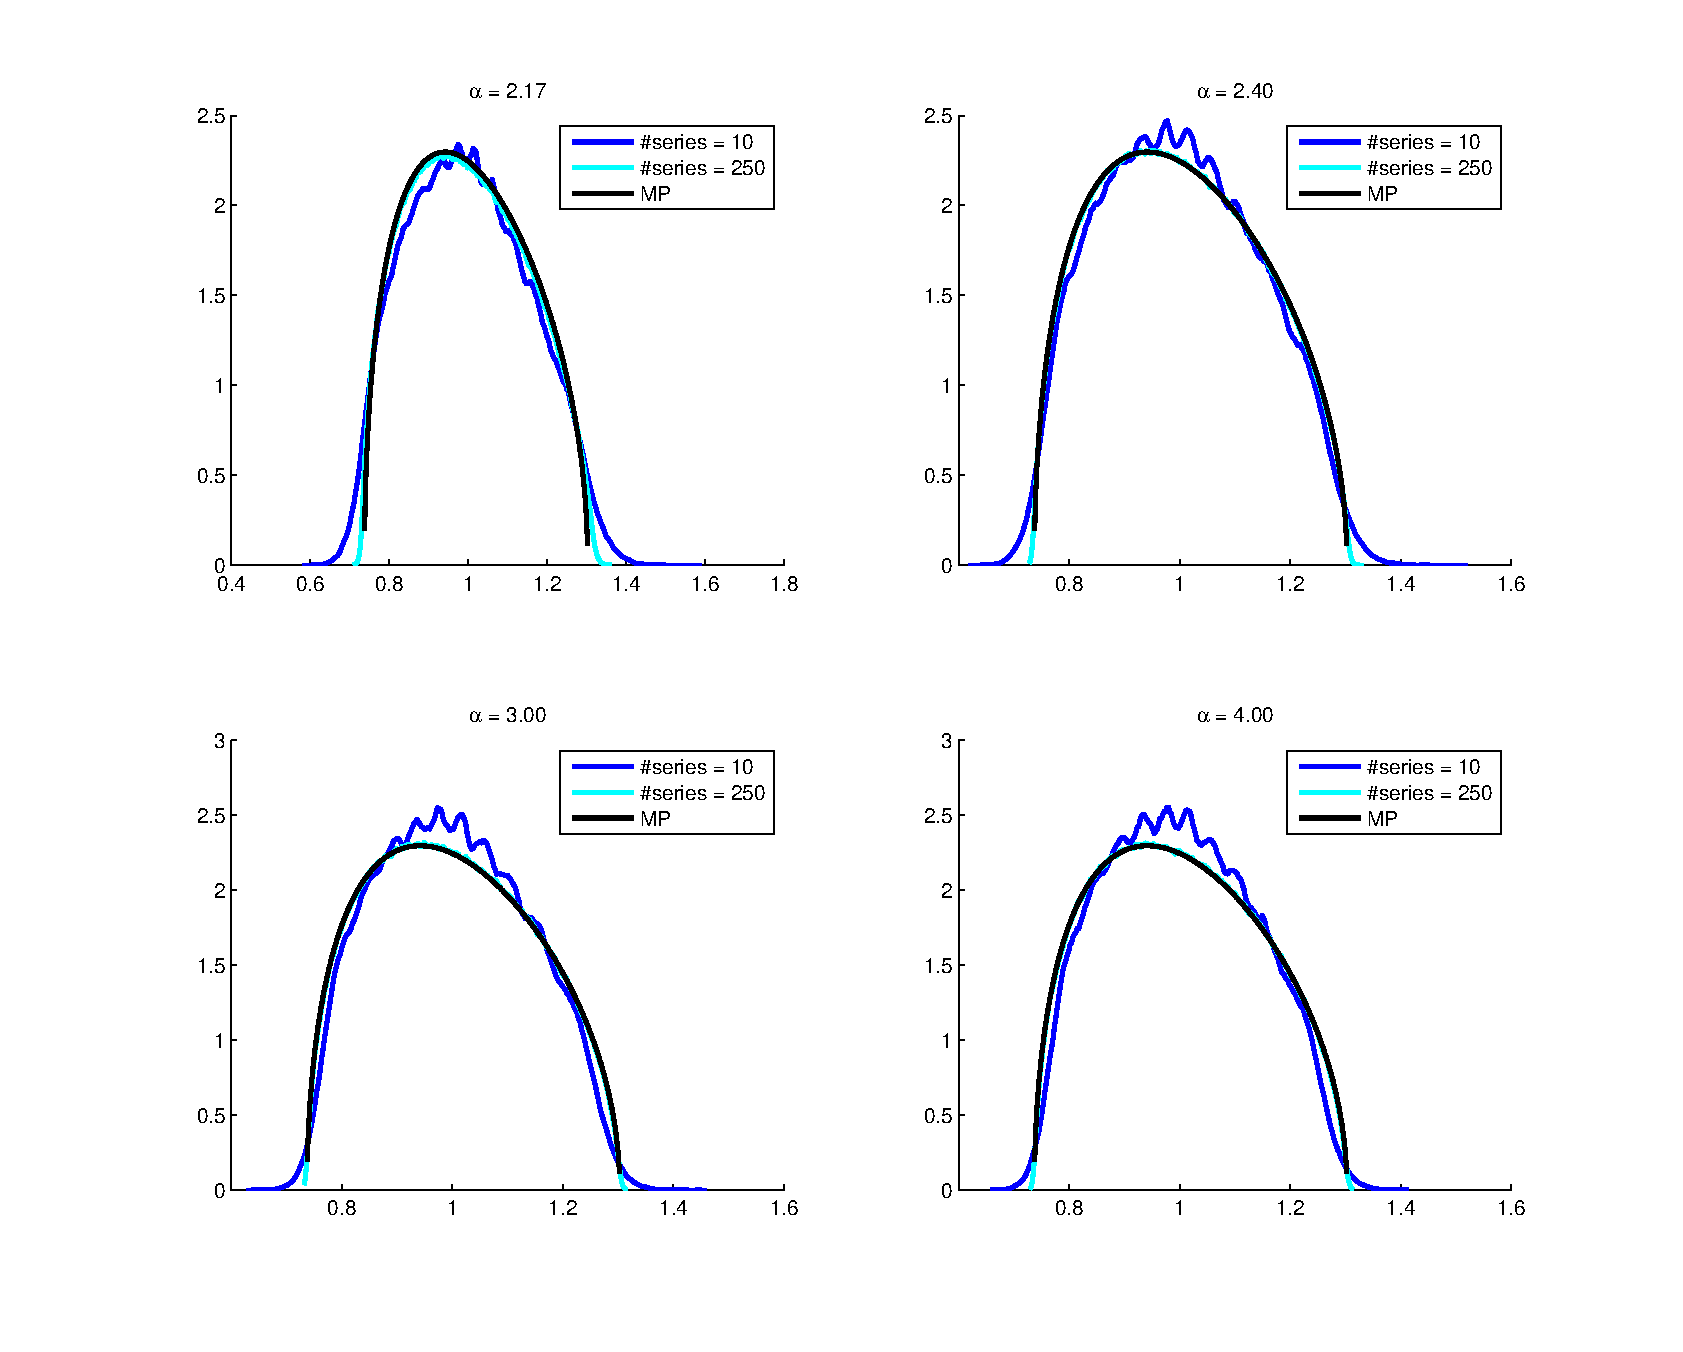
\includegraphics[scale=0.3]{../pics/spectra_q50.eps}
  \caption{\small \it Spectra with q = 50}
\end{figure}

Apparently the spectral density is changed even when the ratio $q$ is left
unchanged by varying $N$ and $T$. For this matter, I notice that for
Burda et al's weighted covariance matrix,
\begin{eqnarray*}
  C &=& {1 \over T} \mtx{RWR'}
\end{eqnarray*}
the spectral density also has $T$ dependence via the parameter $\beta$:
\begin{eqnarray*}
  \beta &=& T(1 - \alpha)
\end{eqnarray*}
where $\alpha$ in their IGARCH(1) model is analogous to $\beta_1$ in a
GARCH(1, 1) model.

\section{Why large deviation from MP at small $\alpha_1$}
Figure \ref{fig:Distance_to_MP} shows that when $\alpha_1$ is small,
deviation of the spectral density from the MP law is large with all
values of the tail exponent $\alpha$. Explanation to this can be found
in the autocorrelations of a GARCH(1,1) process.
\begin{figure}[htb!]
  \centering
    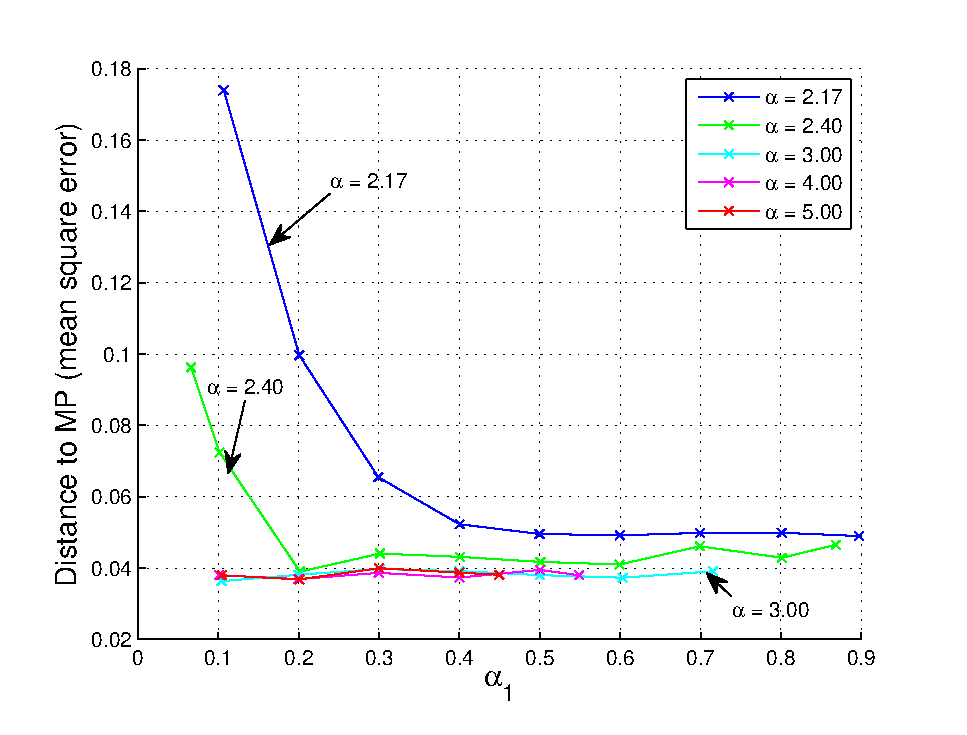
\includegraphics[scale=0.6]{../pics/Distance_to_MP.eps}
    \caption{\small \it Distance of the empirical spectral density to
      the Marchenko-Pastur law measured in terms of the mean square
      error between the two density functions}
    \label{fig:Distance_to_MP}
\end{figure}

A detailed calculation reveals the following autocorrelation
structure for a GARCH(1,1) process:
\begin{eqnarray*}
  \rho_n = \text{corr}(\epsilon_t^2, \epsilon_{t-n}^2) &=& (\alpha_1
  + \beta_1)^{n-1} \rho_1 \\
  \rho_1 = \text{corr}(\epsilon_t^2, \epsilon_{t-1}^2) &=& \alpha_1 +
  \beta_1 - \frac{\beta_1 [1 - (\alpha_1 + \beta_1)^2]}{
    1 - (\alpha_1 + \beta_1)^2 + \alpha_1^2
  }
\end{eqnarray*}
where $n \geq 2$. Figure \ref{fig:autocorr_1} and
\ref{fig:autocorr_1_full} shows $\rho_1$ as a function of $\alpha_1$
and $\beta_1$.
\begin{figure}[htb!]
  \centering
  \subfigure[$\rho_1 = \text{corr}(\epsilon_t^2, \epsilon_{t-1}^2)$ as
  a function of $\alpha_1$ and $\beta_1$. The plot is restricted to a
  region of small $\alpha_1$ and large $\beta_1$ such that $\alpha_1 +
  \beta_1 \approx 1$.]{
    \includegraphics[scale=0.8]{../pics/autocorr_1.pdf}
    \label{fig:autocorr_1}
  }
  \subfigure[$\rho_1 = \text{corr}(\epsilon_t^2, \epsilon_{t-1}^2)$ as
  a function of $\alpha_1$ and $\beta_1$. The plot covers the entire
  region of $\alpha_1 > 0$, $\beta_1 > 0$ and $\alpha_1 + \beta_1 <
  1$. Please ignore the spike, which is due to numerics.]{ 
    \includegraphics[scale=0.5]{../pics/autocorr_1_full.pdf}
    \label{fig:autocorr_1_full}
  }
\end{figure}
It is seen that, as $\alpha + \beta \to 1$, $\rho_1 \to 1$ even if
$\alpha_1$ is rather small. On a curve of constant-$\alpha$, as
$\alpha_1 \to 0$, $\alpha + \beta \to 1$ and hence $\rho_1 \to
1$. Thus for a fixed $\alpha$, very small $\alpha_1$ implies very
strong auto-correlation and hence large deviation of the spectral
density from the MP law.
\end{document}
